\chapter{Installation}

There are two ways to obtain \Peano: 
You can either download one of the archives we provide on the webpage, or you
can work directly against a repository clone (recommended).
If you work with the archive, type in a 
\begin{code}
tar -xzvf myarchive.tar.gz
\end{code}
in the directory where you've stored your downloaded file.


If you work with the git archive, you have to clone this archive first. 
I grant access to \Peano\  free of charge and the repository is public.
However, I ask users to sign up for the software if they indend to push
modifications to the code (which I very much appreciate\footnote{\Peano's
guidebook (the file you currently read) is hosted within \Peano's git
repository, too. I'm always happy if people add content to this
documentation, too.}).
This way I can report to funding agencies how frequent the software is used, and
I also have at least some ideas which application areas benefit from the
software and where it is actively used and developed.
If you do not indend to modify the \Peano\ core code base, you can just clone
the code anomymously.

\begin{code}
git clone https://gitlab.lrz.de/hpcsoftware/Peano.git
cd Peano
git checkout p4
\end{code}


\begin{remark}
I still maintain the ``old'' Peano in the repository (version 3), and most users
consider this to be the standard Peano generation.
For the present document, it is thus important that you manually switch to the
branch \texttt{p4}.
\end{remark}



\section{Prepare the configure environment}

This step should only required if you work directly against the git repository.
If you prefer to download a snapshot of \Peano, then you can skip this section
and continue with \ref{section:installation:configure}.


\begin{itemize}
  \item Ensure you have the autotool packages installed on your system. They
  typically are shipped in the packages \texttt{autoconf}, \texttt{automake} and
  \texttt{libtool}.
  \item Set up the configure environment: 
 \begin{code}
 libtoolize; aclocal; autoconf; autoheader; 
 cp src/config.h.in .; 
 automake --add-missing
 \end{code}
\end{itemize}


\noindent
These steps should only be required once, unless you push major revisions to the
development branch.


\section{Configure}
\label{section:installation:configure}


\Peano\  relies on the autotools to set up its build environment.
Change into the project's directory and type in 
\begin{code}
./configure --help
\end{code}


\noindent
The \texttt{--help} option should give you some information about the available
variants of \Peano.
A sole \texttt{./configure} call gives you the minimalist version of
\Peano---might be appropriate for a first test.

\begin{remark}
 I recommend that you start a first test without any additional flavours of
 \Peano, i.e.~to work with a plain \texttt{./configure} call. Once the tests
 pass, I recommend that you add further options (IO) and/or parallelisation.
 Please note that the baseline config is not sufficient for most applications
 as it is merely a stripped down version of the \Peano\ core.
 \ExaHyPE\ for example requires you to add \texttt{--enable-exahype} and
 \texttt{--enable-loadbalancing-toolbox}. 
 But the bare/minimal version is good for first tests.
\end{remark}


\noindent
The output of \texttt{./configure --help} should be reasonable verbose, but I
summarise some key options below:

\begin{center}
 \begin{longtable}{lp{10cm}}
  \texttt{--with-multithreading} & Switch on multithreading. By default, we
  build without multithreading, but a \texttt{--with-multithreading=cpp}, e.g.,
  makes \Peano\  use the C++ threading model. Please consult \texttt{--help} for
  details. Note: To use OpenMP multithreading, you will need a compiler which
  supports OpenMP 5.0 (e.g - GCC 9.x)\footnote{\Peano\ realises its GPGPU
  offloading via OpenMP, too. Some compilers struggle to translate these GPGPU
  instructions. In this case, please configure with the CXXFLAG
  \texttt{-DnoGPUOffloading}.}.
   \\
  \texttt{--with-mpi} & Enable the MPI version of \Peano. You have to tell the
  build environment however which compile command to use. Please note that
  we need a C++ MPI wrapper. So \texttt{--with-mpi=mpcxx} is a typical call. 
   \\
  \texttt{--with-vtk} & Inform \Peano\  that VTK is available on the system.
  \Peano\ mainly
  relies on its own IO data format. Even some VTK dump routines (used usually
  only for debugging) are written by hand, i.e.~do not rely on the VTK
  libraries.
  However, \Peano\ comes along with some command line conversion tools that can convert its tailored data
  dumps into VTK, and they do rely on the VTK libraries. With this flag, you
  tell \Peano\ to build these tools.
  The VTK installation is sometimes not easy (and you might have to provide additional parameters depending on your installation). I dedicate Chapter \ref{chapter:postprocessing} on VTK.
   \\
  \texttt{--with-hdf5} & Make \Peano\  support HDF5 output. Not stable at the
  moment.
   \\
  \texttt{--with-delta} & Configure \Peano\  such that the geometry library
  $\Delta $ is used. Not stable at the moment.
   \\
  \texttt{--with-toolchain} & Build against a particular vendor toolchain.
  Currently, I have dedicated support for the NVIDIA NVTX SDK
  (\texttt{--with-toolchain=nvidia}) providing NVIDIA-specific logging/tracing
  as well as memory allocation calls---the latter is of use if you use
  GPUs---and the Intel toolchain (\texttt{--with-toolchain=intel}). The latter
  in particular links against the ITAC tracing API. I also have support for
  Google's Chrome browser (\texttt{--with-toolchain=chrome}) which means that
  traces are written in a way that you can display it in Chrome. Ensure that your CXXFLAGS set the right include path\footnote{It is
  \texttt{CXXFLAGS+=-I/opt/nvidia/nsight-systems/2020.3.1/target-linux-x64/nvtx/include/nvtx3/}
  on my system, e.g.}.
  This is optional.
   \\
  \texttt{--with-gpu} & Add GPGPU support. Depending on the target, we currently
  have specialised versions for NVIDIA (\texttt{--with-gpu=nvidia}) and AMD
  (\texttt{--with-gpu=amd}). For different vendors, you might be required to
  select particular multithreading models. The AMD and NVIDIA port for example
  work only with OpenMP.
   \\
  \texttt{--enable-exahype} & Includes the \ExaHyPE\ core into your build.
   Requires the load balancing toolbox, too. 
   \\
  \texttt{--enable-xxx-toolbox} & \Peano\ is shipped with a couple of toolboxes
   for various purposes. These are C++ libraries which offer a lot of features.
   You have to enable/activate them manually. Please note: Not all toolboxes are
   compatible with all targets. We have experienced issues with the
   FEM toolbox and some GPGPU systems for example.
 \end{longtable}
\end{center}




\noindent
Compilers, linkers and both compiler and linker flags can be changed by
resetting the corresponding environment variables (such as
\texttt{CXX} or \texttt{LDFLAGS} or \texttt{CCFLAGS}) \emph{prior} to the
configure call.
Alternatively, you can pass the variables to be used to \texttt{configure}
	through arguments (\texttt{./configure CXX=icpc ...}, e.g.). 
Please consult the \texttt{--help} output for details.
For some supercomputers that we use frequently, there are recommendations which
setting to use (Chapter~\ref{chapter:selected-HPC-platforms}).


\begin{remark}
Most Linux tools prefer you to specify a dedicated installation directory via
\texttt{--prefix}.
For \Peano, things are slightly different: \Peano\ is a mere engine, i.e.~not
``useful'' per se.
It is applications built on top of \Peano\ that become tools that you might
later want to install/deploy on your system. 
Therefore, I ship \Peano\ with static libraries only, and most users work with
the code in the download/installation directory until they have constructed the
application with the help of \Peano.
So no need to specify a proper installation directory via \texttt{--prefix}.
\end{remark}


%   \texttt{--prefix=/mypath} & Will install \Peano\  in \texttt{/mypath}.
%    \\


\section{Build}

Once the configuration has been successful, a simple 
\begin{code}
make
\end{code}
should build the \Peano\ core.
It also builds some examples and all the extensions and toolboxes you have
manually enabled.
All of these go into static libraries.
The code is not small and you thus might prefer
\begin{code}
make -jx
\end{code}
with x being the number of parallel builds to use.


\begin{remark}
 Following up on the remark above, 
 \begin{code}
make install
 \end{code}
 would deploy the \Peano\ files in the directory specified via the
 \texttt{prefix} before.
 Most Unix tools want you to install them. 
 For \Peano, things might be slightly different as it is an engine used to
 construct tools in the first place. 
\end{remark}





\section{Installation test}

Once you have compiled \Peano\, I recommend that you run all tests using

\begin{code}
  make check
\end{code}

\noindent
The call launches all of \Peano's unit test, i.e.~all the unit tests for the
core plus the extensions that you have enabled.


\begin{remark}
 I have written the test target such that it works out-of-the-box for non-MPI
 calls. If you have configured with \texttt{--with-mpi}, then the unit tests
 will fail. But this does not mean that the unit tests are broken. It is simply
 due to the fact that the makefile's test target does not know that you have to
 use the \texttt{mpirun} prefix.
 To make a long story short: If you use MPI and you want to run the unit tests,
 you have to do so manually.
\end{remark}


\noindent
To run 2D and 3D tests individually, use

\begin{code}
  src/unittests/UnitTests2d
  src/unittests/UnitTests3d
\end{code}

\noindent
You can run these builds with different core counts and also MPI support if you
have compiled with MPI.
The executables contain both node correctness tests and MPI ping-pong tests,
i.e.~you can both assess a valid build plus a working MPI environment.
If successful, you should always get a message alike

\begin{code}
Peano 4 (C) www.peano-framework.org 
build: 2d, with mpi (1 ranks), omp (4 threads), debug level=4
it is recommended that you run the unit tests with more than one MPI rank, too (file:main.cpp,line:82)
usage: ././UnitTests2d core-count (use default core count=1 now) (file:main.cpp,line:88)
running test case collection "tarch.la.tests" ..... ok
running test case collection "tarch.la" ............. ok
running test case collection "tarch.mpi.tests" ..... ok
running test case collection "tarch.mpi" ... ok
running test case collection "tarch" ... ok
running test case collection ... ok
running test case collection "peano4.grid.tests" ....... ok
running test case collection "peano4.grid" ... ok
running test case collection "peano4.parallel.tests" ....... ok
running test case collection "peano4.parallel" ... ok
running test case collection "peano4" ... ok
running test case collection ... ok
\end{code}

\noindent
Watch out for the last line that tells you whether the overall unit tests passed
through.

\section{Python configuration}

\Peano\ is developed with Python 3. Python 2 is not supported. 


\subsection{Python paths}
To make any Python example pass, you have to set the Python paths.
There are multiple ways to do so.

The standard way is to set the \texttt{PYTHONPATH}:
\begin{code}
export PYTHONPATH=myPeanoDirectory/python
\end{code}
This can even be done in the \texttt{.bashrc}.

Alternatively, you can augment your Python scripts later on with 
\begin{code}
import sys
PEANO4_PYTHON_DIR="myPeanoDirectory/python"
sys.path.append(PEANO4_PYTHON_DIR)
\end{code}


\noindent
Please note that most Python scripts require you to set the
\texttt{LD\_LIBRARY\_PATH}. 
If you install \Peano, then this path should be automatically right.
If you work with a local \Peano\ installation, you can either tell \Peano\
through its API where to search for the library (all routines that add a
library accept additional search paths), or you can again use the
\texttt{sys.path.append} command to extend \texttt{LD\_LIBRARY\_PATH}.


\begin{remark}
 I personally prefer the variant to go through the environment variable.
 \Peano's Python API yield plain old makefiles building executables that work
 completely without any Python. 
 This way, we ensure that we work smoothly on supercomputers, too, where Python
 sometimes is not available in the latest version or on the compute nodes.
 As long as you run through environment variables or the \Peano\ routines to
 specify paths, your makefiles also will continue to work that way. 
\end{remark}


\subsection{Python packages}

\Peano\ currently relies on the following Python packages/projects:


\begin{center}
 \begin{tabular}{lp{6cm}ll}\\
   Package & Description & Ubuntu & OpenSUSE \\
   \hline
   jinja2 & For all the templated glue code. & 
    \texttt{python3-jinja2} &
    \texttt{} 
    \\
   sympy & For the symbolic modelling of partial differential equations
    (predominantly in \ExaHyPE). &
    \texttt{python3-sympy} &
    \texttt{python3-sympy} 
 \end{tabular}
\end{center}


\noindent
The table above specifies the corresponding packages in our two main
distributions for which we test \Peano. 
They can be installed via \texttt{zypper install} (SUSE) or \texttt{apt-get
install} (Ubuntu), respectively.
Alternatively, you might want to use Python's \texttt{pip}.





\section{Fortran}

\begin{remark} 
 If you don't use Fortran in your own code, ignore this section.
\end{remark}

\Peano's core does not use any Fortran at all. 
However, many users use Fortran for their domain-specific programming.
If you want to have a seemless integration of your particular Fortran choice
through \Peano's Python API, invoke \texttt{./configure} ensuring that the
Fortran variables---in particular the environment variable \texttt{FC}
identifying the compiler---are properly set.


For many codes and the GNU Fortran compiler, you need the flag
\texttt{-fdefault-real-8}.
You can export \texttt{FCFLAGS} and make it contain this argument before you
invoke \texttt{configure}.
As the \Peano's core does not use Fortran---it is only applications built on top
of \Peano---you can redefine the flags later on (see \ref{section:installation:applications-built-with-Peano}).



\section{\Peano\ components and build variants}
\label{chapter:installation:build-variants}

\Peano\ currently is delivered as a set of archives, i.e.~static libraries:
\begin{itemize}
  \item There is a technical architecture (\texttt{Tarch}) and the actual
  \texttt{Peano4Core}.
  \item Each archive variant is available as a release version, as a debug
  version, as a version with tracing and assertions and as a tracing-only
  version.
  \item Each archive variant is available as 2d build and as 3d build. If you
  need higher dimensions, you have to build the required libraries manually.
\end{itemize}


The version terminology is as follows:
\begin{itemize}
  \item {\bf debug} The debug versions of the archives all have the postfix
  \texttt{\_debug}. If you link against these versions, the full set of
  assertions, of all tracing and all debug messages is available; though you can
  always filter on the application-level which information you want to see
  (cmp.~Chapter \ref{section:logging}).
  \item {\bf asserts} Thsee versions of the archives all have the postfix
  \texttt{\_asserts}. If you link against these versions, all assertions are on.
  The code also contains tracing macros (see below).
  \item {\bf tracing} The release versions of the archives all have the postfix
  \texttt{\_trace}. If you link against these versions, all assertions and debug
  messages are removed, but some tracing is active. You can switch on/off the
  tracing per class (cmp.~Chapter \ref{section:logging}), and different tracing
  backends allow you to connect to different (profiling) tools.
  \item {\bf release} The release versions of the archives have no
  particular postfix. They disable tracing, any debugging and all assertions.
  These archives should be used by production runs.
\end{itemize}


\begin{remark}
 Peano's release components still write info messages (they suppress debug,
 tracing and logging, but not essential information). If you want to filter out
 these messages, too, you have to apply a log filter (Chapter
 \ref{section:logging:log-filter}).
\end{remark}


\noindent
Besides these archives, the \Peano\ installation also comes along with a set of
example applications.
They are found in the directory \texttt{src/examples}.
Most examples create by default two variants of the example: a debug
version and one with only tracing enabled.
Several examples furthermore come along as 2d and 3d build.



\section{Documentation}

\begin{figure}
 \begin{center}
  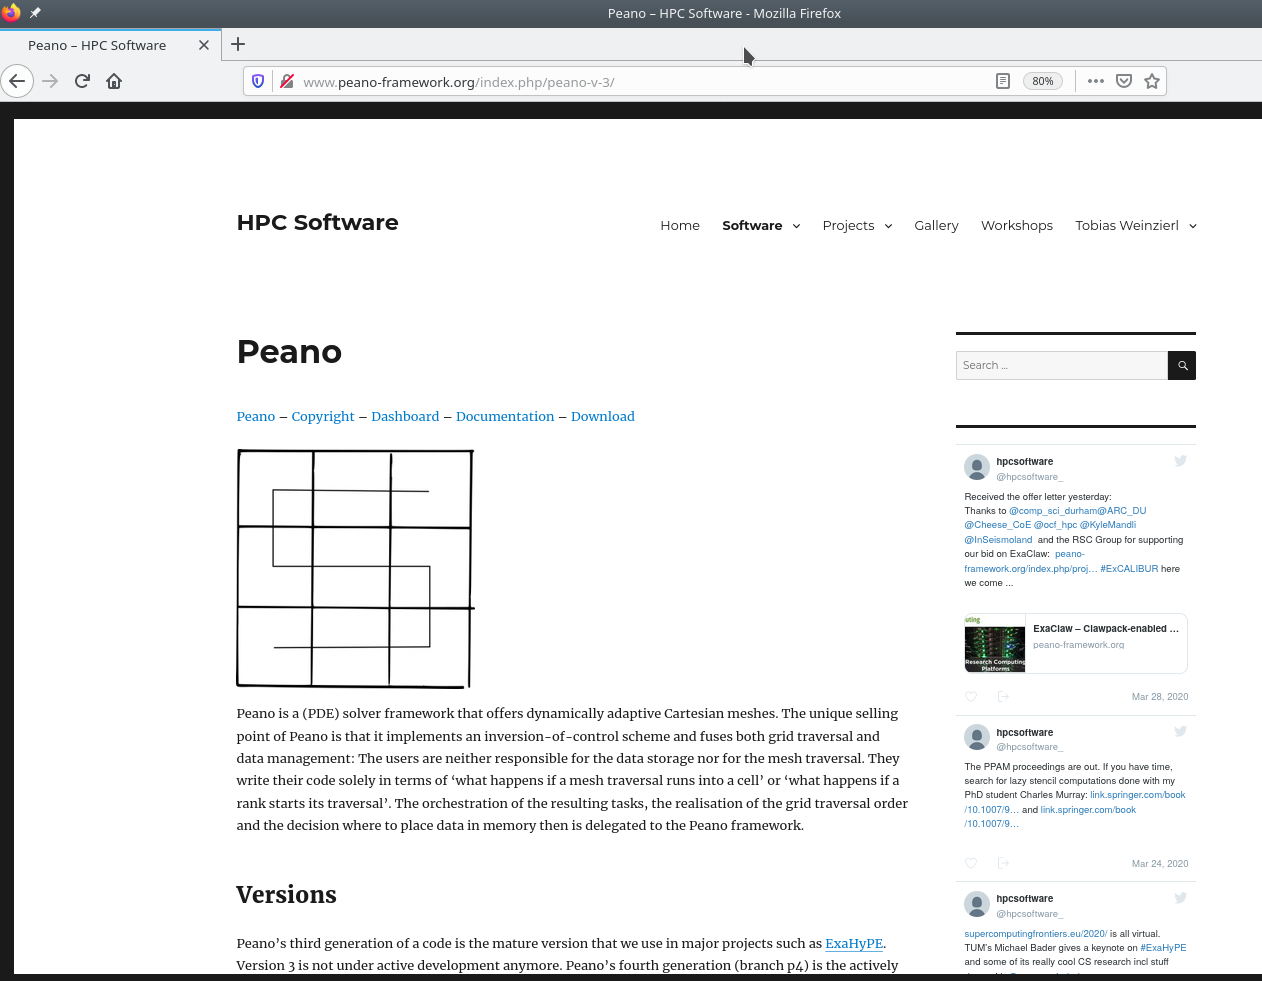
\includegraphics[width=0.4\textwidth]{10_installation/webpage.png}
  \hspace{0.4cm}
  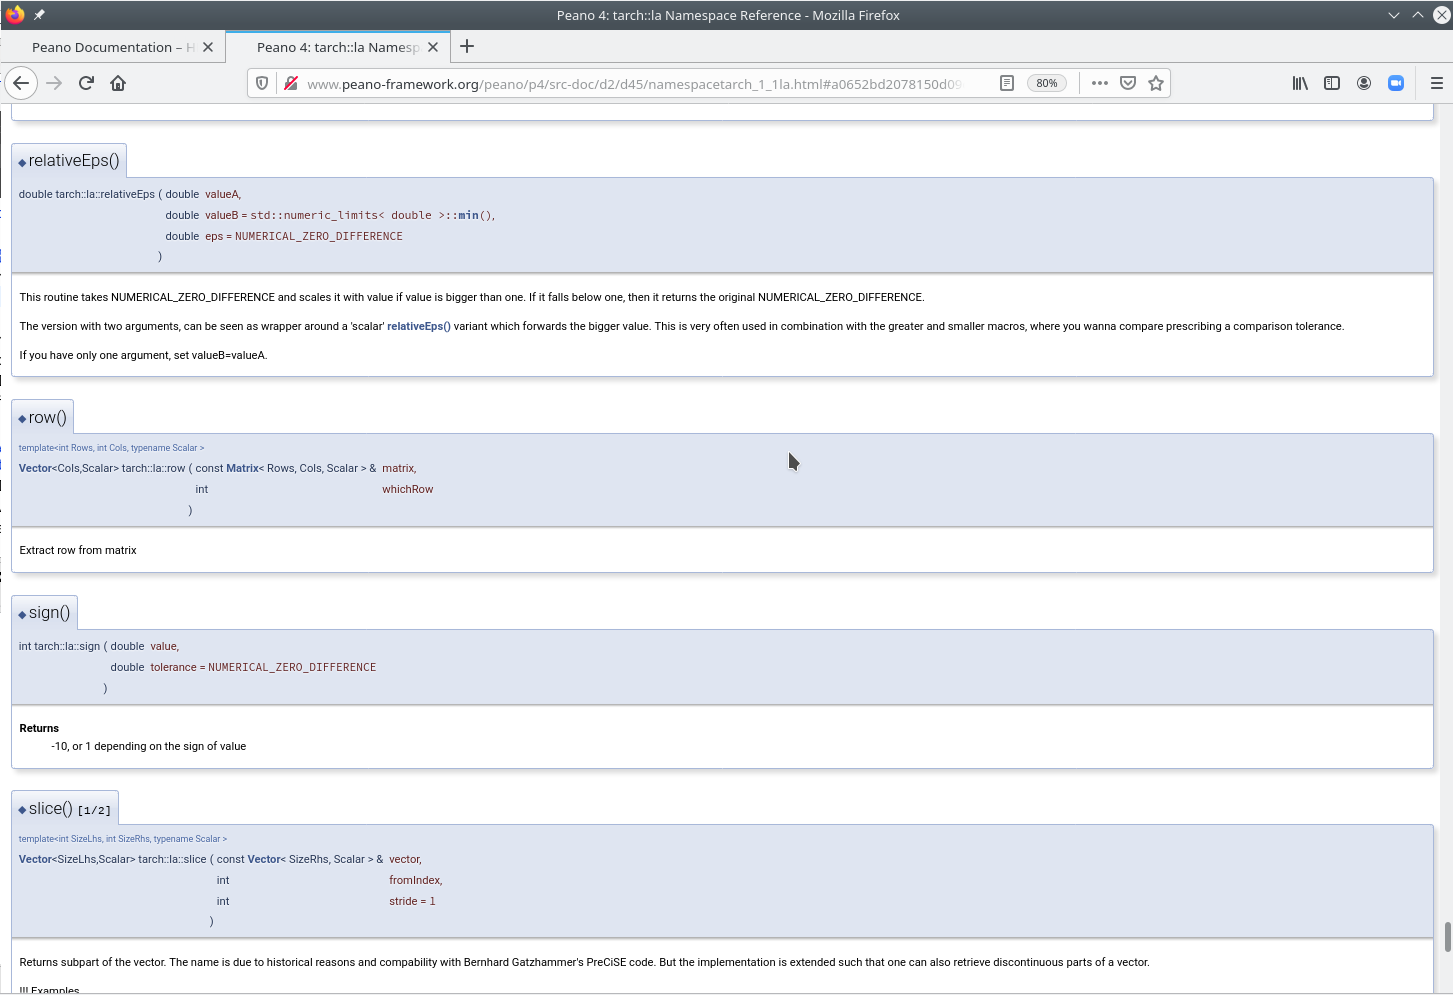
\includegraphics[width=0.4\textwidth]{10_installation/source-docu.png}
 \end{center}
 \caption{
  \Peano's webpage (left) and a screenshot from the auto-generated source code
  docu which can be reached through the webpage if you don't want to generate
  the pages yourself.
  This documentation also provides indices and a search function as well as all
  documentation formulae typeset with LaTeX.
 }
\end{figure}



There are three major types/resources of documentation of the software:
\begin{enumerate}
  \item This guidebook/cookbook that describes how to use the code base from a
  high abstraction level and with anecdotal examples.
  \item The documentation of the C++ code. Here, I follow an ``everything is in
  the code'' philosophy.
  \item The documentation of the Python code. Here, I follow an ``everything is
  in the code'' philosophy.
\end{enumerate}

\noindent
For the code documentation, ``everything is in the code'' means that all
documentation is comments within the Python script or C++ header files,
respectively.
You can create a webpage from this distributed information through
the tool \texttt{doxygen}\footnote{\url{http://www.doxygen.nl}.}. 


There are two Doxygen configuration files in the repository, i.e.~I keep the
Python and the C++ documentation output separate.
To create the documentation, switch into directory \texttt{src} or
\texttt{python}, respectively. 
In both directories, the Doxygen config file is called
\texttt{peano.doxygen-configuration}, i.e.~calling

\begin{code}
doxygen peano.doxygen-configuration
\end{code}

\noindent
gives you the output. If you prefer not to generate and maintain the
documentation yourself, the \Peano\ webpage hosts the autogenerated
documentation, too.
It is updated roughly once a week.



\section{Compile/link options for applications built with \Peano}
\label{section:installation:applications-built-with-Peano}

\Peano\ is a framework, i.e.~ships very few executables (mainly only for test
purposes and for postprocessing).
Its core delivery is a set of libraries.
Application codes then build on top of these libraries.
While it is up to you to decide which build system you use in your application,
\Peano\ natively favours makefiles.


If you use \Peano's Python API, it will create dummy makefiles.
Higher-level \Peano\ applicaitons such as \ExaHyPE\ build upon the Python API
and thus work with makefiles, too.
When they create these makefiles, they parse your local \Peano\ installation's
makefiles and extract the information from there.
This is, when you've selected a particular compiler or compiler option when you
install \Peano, this choice will automatically propagate through to your
domain-specific codes.
There's however the option to overwrite the chosen settings---either by defining
appropriate environment variables before you invoke \texttt{make} or by
resetting variables manually within your Python scripts that configure the
environment.



